\documentclass[12pt,a4paper]{article}
% Estilo compartido para informes. Compilar con LuaLaTeX desde tp1/.
\usepackage[spanish,es-nodecimaldot]{babel}
\usepackage{fontspec}
\setmainfont{Montserrat-Medium.ttf}[
  Path=../assets/fonts/,
  BoldFont=Montserrat-Bold.ttf,
  ItalicFont=Montserrat-MediumItalic.ttf]
\usepackage[a4paper,margin=2.5cm,headheight=16pt]{geometry}
\usepackage{xcolor,graphicx,booktabs,tabularx}
\usepackage{float}
\usepackage{titlesec,fancyhdr,enumitem,caption}
\usepackage{ragged2e}
\usepackage{hyperref}
\definecolor{verde}{HTML}{1D4036}
\definecolor{bronce}{HTML}{D38129}
\definecolor{rosa}{HTML}{D88E77}
\definecolor{calido}{HTML}{EFE4D8}
\definecolor{grafito}{HTML}{1D1D1D}
\hypersetup{colorlinks=true,linkcolor=verde,urlcolor=verde,
  pdftitle={TP1 - Instalación de máquinas virtuales},pdfsubject={Cyberseguridad}}
\AtBeginDocument{\color{grafito}\RaggedRight\fontsize{12}{14.4}\selectfont}
\setlength{\parindent}{0pt}
\setlength{\parskip}{7pt}
\setlist[itemize]{leftmargin=*,itemsep=7pt,topsep=4pt}
\setlist[enumerate]{leftmargin=*,itemsep=6pt}
\titleformat{\section}{\color{verde}\bfseries\fontsize{18}{21.6}\selectfont}{\thesection}{0.65em}{}
\titleformat{\subsection}{\color{verde}\bfseries\large}{\thesubsection}{0.65em}{}
\titleformat{\subsubsection}{\color{verde}\bfseries}{\thesubsubsection}{0.65em}{}
\titlespacing*{\section}{0pt}{16pt}{8pt}
\titlespacing*{\subsection}{0pt}{12pt}{5pt}
\titlespacing*{\subsubsection}{0pt}{10pt}{4pt}
\setcounter{tocdepth}{2}
\pagestyle{fancy}
\fancyhf{}
\fancyhead[L]{\small\color{verde}FCEFyN | UNC}
\fancyhead[R]{\small\color{verde}\materia\ · TP \numeroTP}
\fancyfoot[L]{\scriptsize Informe de laboratorio}
\fancyfoot[R]{\small\thepage}
\renewcommand{\headrulewidth}{0.4pt}
\captionsetup{font=small,labelfont=bf,justification=raggedright,singlelinecheck=false,hypcap=false}
\newcommand{\pendiente}[1]{\par{\small\color{verde}\textbf{Por completar.} #1\par}}
% Si falta una captura se muestra un espacio reservado; no impide compilar.
\newcommand{\captura}[2]{%
  \par\smallskip\begingroup\centering
  \IfFileExists{figuras/#1}{%
    \includegraphics[width=\linewidth,height=5cm,keepaspectratio]{figuras/#1}%
  }{%
    \setlength{\fboxsep}{10pt}%
    \fcolorbox{bronce}{calido}{\parbox[c][1.25cm][c]{\dimexpr\linewidth-2\fboxsep-2\fboxrule\relax}{%
      \centering\small Captura pendiente\par\texttt{\detokenize{#1}}}}%
  }%
  \captionof{figure}{#2}\par\endgroup\smallskip
}

\usepackage{xurl}

\newcommand{\materia}{Cyberseguridad}
\newcommand{\numeroTP}{6}
\newcommand{\tituloTP}{Uso de tcpdump}
\newcommand{\estudiante}{Brigido Tomas Andres}
\newcommand{\legajo}{38481096}
\newcommand{\carrera}{ICOMP}
\newcommand{\docente}{Javier A. Jorge}


% Metadatos específicos del TP6 y capturas en img/.
\hypersetup{pdftitle={TP6 - Uso de tcpdump}}
\renewcommand{\captura}[2]{%
  \begin{figure}[H]
    \centering
    \IfFileExists{img/#1}{%
      \includegraphics[width=0.85\linewidth,height=5cm,keepaspectratio]{img/#1}%
    }{%
      \setlength{\fboxsep}{10pt}%
      \fcolorbox{bronce}{calido}{\parbox[c][1.1cm][c]{0.85\linewidth}{%
        \centering\small Captura pendiente\par\texttt{\detokenize{#1}}}}%
    }%
    \caption{#2}
  \end{figure}
}

\begin{document}
\hypersetup{pageanchor=false}
\begin{titlepage}
  
\includegraphics[width=8cm]{../assets/logo-fcefyn-2026.png}
  \vspace{1cm}

  {\color{verde}\small UNIVERSIDAD NACIONAL DE CÓRDOBA\par}
  \vspace{2.1cm}
  {\color{bronce}\bfseries\large TRABAJO PRÁCTICO \numeroTP\par}
  \vspace{0.45cm}
  {\color{verde}\bfseries\fontsize{32}{38.4}\selectfont Uso de\\tcpdump\par}
  \vspace{0.3cm}
{\small Captura y análisis de tráfico de red\par}
\vspace{0.35cm}
  {\large \materia\par}
  \vspace{0.8cm}
  {\color{bronce}\rule{2.7cm}{2pt}\par}
  \vfill
  \renewcommand{\arraystretch}{1.45}
  \begin{tabular}{@{}p{3.2cm}p{10cm}@{}}
    Estudiante & \estudiante \\
    Legajo & \legajo \\
    Carrera & \carrera \\
    Docente & \docente \\
  \end{tabular}
  \vfill
  {\small Córdoba, Argentina\par}
\end{titlepage}
\hypersetup{pageanchor=true}

\tableofcontents
\vspace{1cm}
\newpage

\section{Introducción y objetivos}
Este trabajo propone aprender a utilizar \texttt{tcpdump} para observar tráfico desde la terminal, probar sus principales opciones y documentar los resultados mediante capturas de pantalla.

\section{Pruebas y capturas}
Primero identificamos la direccion ip de nuestra interfaz de red con el comando \texttt{ip a}.

\begin{figure}[H]
    \centering
    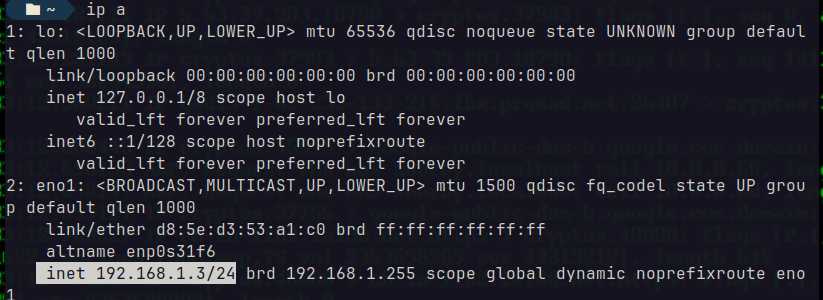
\includegraphics[width=0.9\textwidth]{img/ip.png}
    \caption{Dirección IP de la interfaz de red.}
    \label{fig:captura-dns}
\end{figure}

\subsection{Interfaces y captura}
\begin{verbatim}
tcpdump --version
sudo tcpdump -D
sudo tcpdump -i eno1 -nn -c 30 -v -e -X
\end{verbatim}

\begin{figure}[H]
    \centering
    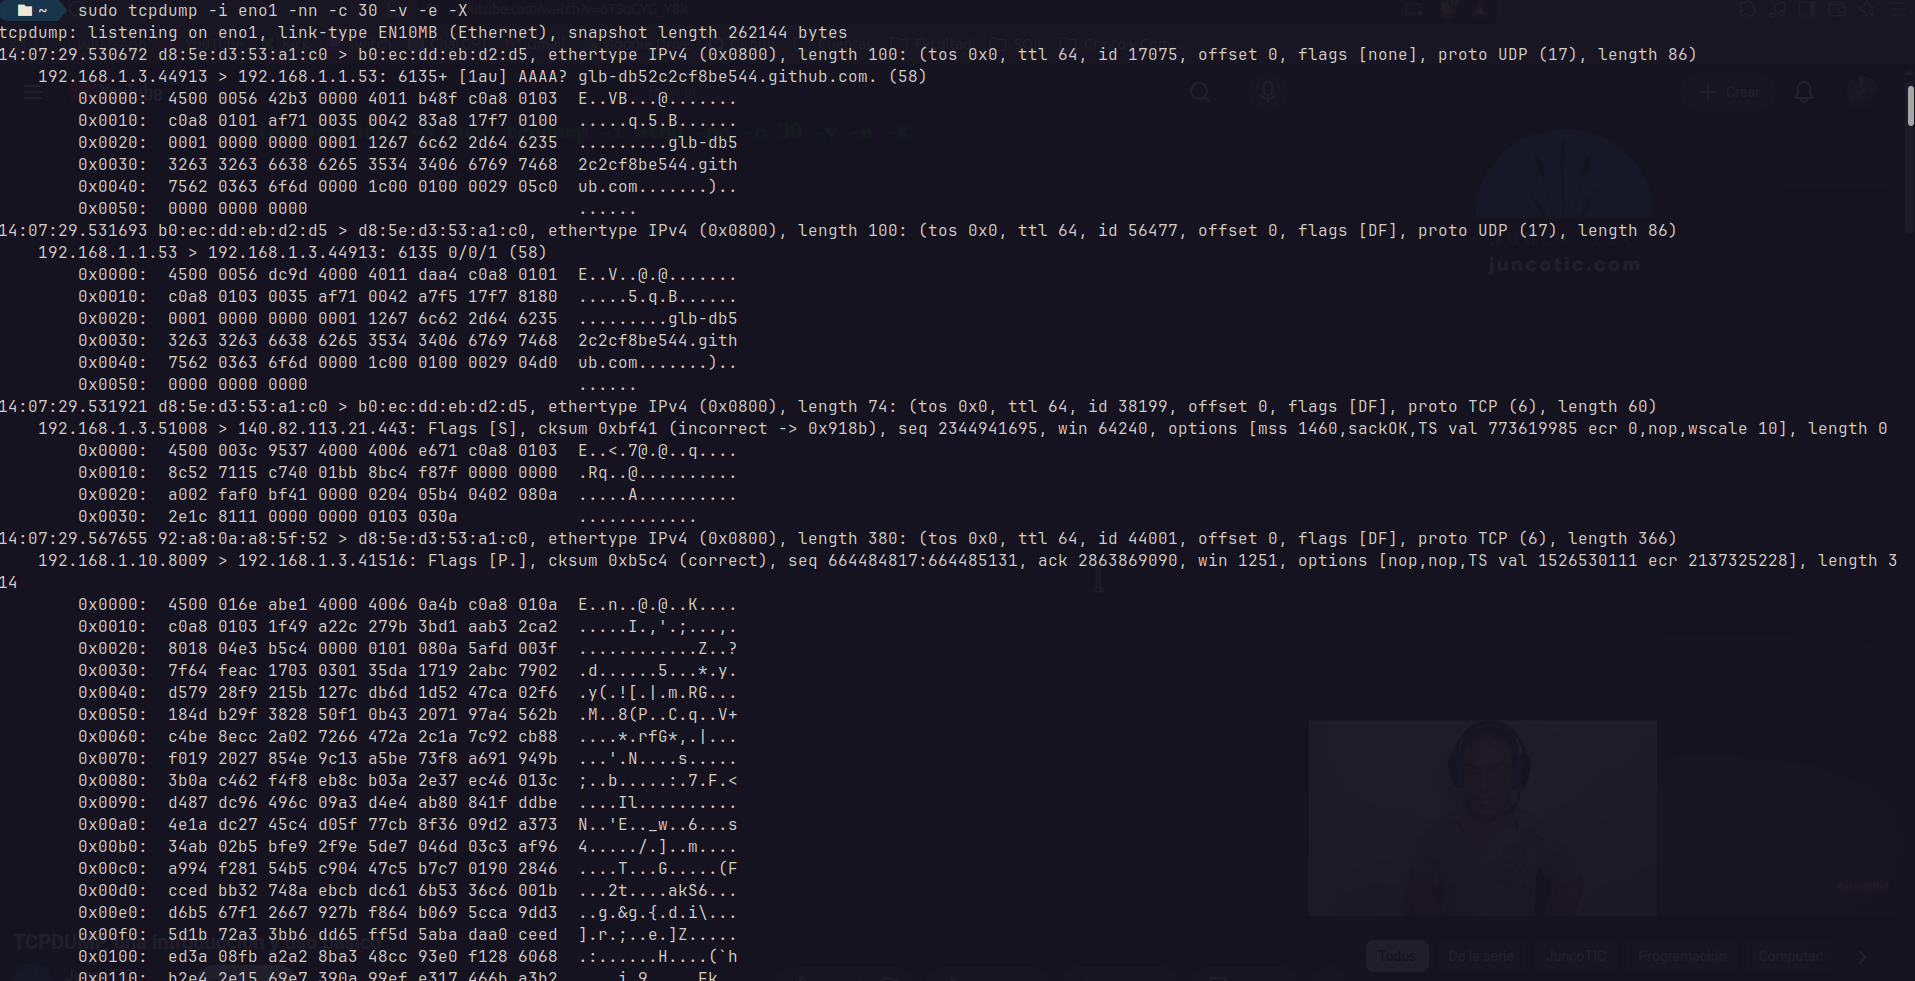
\includegraphics[width=0.9\textwidth]{img/comandolargo.png}
    \caption{Salida del comando tcpdump.}
    \label{fig:captura-dns}
\end{figure}

\section{Flags principales}
\begingroup
\small\renewcommand{\arraystretch}{1.35}
\begin{tabularx}{\linewidth}{@{}>{\ttfamily\RaggedRight\arraybackslash}p{3.2cm}X@{}}
\toprule
\normalfont\textbf{Flag} & \textbf{¿Para qué sirve?} \\
\midrule
-D & Lista interfaces disponibles. \\
-i interfaz & Selecciona la interfaz de captura. \\
-n & Evita resolver direcciones a nombres. \\
-nn & Evita también convertir puertos a nombres de servicios. \\
-c cantidad & Finaliza tras procesar esa cantidad de paquetes. \\
-v, -vv, -vvv & Aumentan progresivamente el detalle mostrado. \\
-e & Incluye el encabezado de enlace, como las MAC en Ethernet. \\
-q & Muestra información resumida. \\
-A & Muestra contenido en ASCII, sin el encabezado de enlace. \\
-X & Muestra contenido hexadecimal y ASCII, sin el encabezado de enlace. \\
-s bytes & Limita los bytes capturados por paquete. \\
-w archivo & Guarda paquetes en un archivo de captura. \\
-r archivo & Lee paquetes de una captura guardada. \\
-t & Omite la marca de tiempo. \\
-tttt & Muestra fecha y hora. \\
\bottomrule
\end{tabularx}
\endgroup

\subsection{Guardar y leer una captura}
\begin{verbatim}
sudo tcpdump -i eno1 -nn -c 30 -v -e -X -w /tmp/captura.pcap
\end{verbatim}

\begin{figure}[H]
    \centering
    
\includegraphics[width=0.9\textwidth]{img/captura.png}
    \caption{Captura de tráfico.}
    \label{fig:captura-dns}
\end{figure}

La captura de trafico se guarda en el formato .pcap, que puede ser leido con el comando \texttt{tcpdump -r /tmp/captura.pcap} y se pueden aplicar los mismos filtros.

% Para otra prueba, duplicar un bloque de comando, captura y explicación.
\section{Filtro avanzado de tráfico}
Los filtros seleccionan qué paquetes capturar o leer de un archivo. Se escriben después de las opciones de \texttt{tcpdump}.

\begingroup
\small\renewcommand{\arraystretch}{1.3}
\begin{tabularx}{\linewidth}{@{}>{\ttfamily\RaggedRight\arraybackslash}p{4.5cm}X@{}}
\toprule
\normalfont\textbf{Filtro} & \textbf{Función} \\
\midrule
src / dst & Selecciona origen o destino; sin ellos, se consideran ambos. \\
host 192.168.1.3 & Filtra por equipo. \\
net 192.168.1.0/24 & Filtra por red. \\
port 53 & Filtra por puerto. \\
portrange 1000-2000 & Selecciona un rango de puertos, incluidos sus extremos. \\
greater 500 & Selecciona paquetes de 500 bytes o más. \\
less 100 & Selecciona paquetes de 100 bytes o menos. \\
not & Excluye lo que cumple la condición. \\
and / or & Exige ambas condiciones o al menos una. \\
\bottomrule
\end{tabularx}
\endgroup

\par\textbf{Ejemplos de uso.}
Tráfico originado en un equipo y dirigido al puerto 53:
\begin{verbatim}
sudo tcpdump -i eno1 -nn 'src host 192.168.1.3 and dst port 53'
\end{verbatim}

Excluir un rango de puertos:
\begin{verbatim}
sudo tcpdump -i eno1 -nn 'not portrange 1000-2000'
\end{verbatim}

Combinar puertos y tamaño mediante paréntesis:
\begin{verbatim}
sudo tcpdump -i eno1 -nn '(port 80 or port 443) and greater 500'
\end{verbatim}

Los paréntesis agrupan condiciones. Dentro de comillas simples no necesitan escape; fuera de ellas se escriben como \verb|\(| y \verb|\)|. Los corchetes y llaves de la imagen representan opciones, no se escriben literalmente.

\newpage
\section{Referencias}
The Tcpdump Group. \href{https://github.com/the-tcpdump-group/libpcap/blob/master/pcap-filter.manmisc.in}{Manual de filtros pcap-filter}.
\par
The Tcpdump Group. \href{https://github.com/the-tcpdump-group/tcpdump/blob/master/tcpdump.1.in}{Manual oficial de tcpdump}. También disponible localmente mediante \texttt{man tcpdump}.
\par Video de YouTube seguido durante la práctica: \url{https://www.youtube.com/watch?v=6TSqCYG_Y8k}.
\par Video de YouTube complementario: \url{https://www.youtube.com/watch?v=uxmd8H9mbLI}.
\end{document}
